\documentclass[a4paper,11pt,ceqn]{article}

%%%%%%%%%%%%%%%%
% Instructions %
%%%%%%%%%%%%%%%%
% Set the document class and settings to match the final document that these figures will be included into
% This will output a pdf with a page for each figure, nicely cropped according to picture dimenstions as defined below in the `Figure' Section. Inlcude in the final document by using package 'graphicx' and command \includegraphics[page=<page of figure>]{figures.pdf}
% The following package is used to create the cropping mentioned above, and apparently should be the last loaded package: \usepackage[active,tightpage]{preview}
% The following command re-writes the figure enviroment to become a preview enviroment - without this spacing is off, and captions and labels may appear
%\renewenvironment{figure}[1][]{%
%	\begin{preview}%
%		\renewcommand{\caption}[2][]{}}
%	{\end{preview}}

%%%%%%%%%%%%%%%%%
% Load Packages %
%%%%%%%%%%%%%%%%%
\usepackage{epsfig}
\usepackage{amssymb}
\pagestyle{empty}
\usepackage{epstopdf}
\usepackage{mathrsfs}
\usepackage{amsmath}
\usepackage{graphicx}
\usepackage{array}
\usepackage{xcolor}    % \nopagecolor
\usepackage{fp}
\usepackage{bm}    % boldmath \bm{}
\usepackage[pdftex,active,tightpage]{preview}    % should be loaded lasts
% adjust borders added to figures: left, lower, right and upper borders. - useful to increase lower border not to cut off labels placed below figure bounds. 
\renewcommand{\PreviewBbAdjust}{0mm -0.25mm 0mm 0mm}
\renewenvironment{figure}[1][]{%
	\begin{preview}%
		\renewcommand{\caption}[2][]{}}
	{\end{preview}}

\setlength{\unitlength}{1cm}

%%%%%%%%%%%%%%%%%%%%%%%%%%%%%%%%%%%%%%%%%%%%%%%%
% Get various dimensions for the documentclass %
%%%%%%%%%%%%%%%%%%%%%%%%%%%%%%%%%%%%%%%%%%%%%%%%
\makeatletter
\newcommand*{\getlength}[1]{\strip@pt\dimexpr0.035136\dimexpr#1\relax\relax}
\newcommand{\showfont}{%
encoding: \f@encoding{},\\
family: \f@family{},\\
series: \f@series{},\\
shape: \f@shape{},\\
size: \f@size{} pt,\\
text height: \getlength{\the\textheight} cm,\\
text width:     \getlength{\the\textwidth} cmx}
\makeatother

\begin{document}

%%%%%%%%%%%%%%%%
%%% Figure 1 %%%
%%%%%%%%%%%%%%%%

\nopagecolor
\begin{figure}
	\begin{picture}(13,7.5)(0,-0.5)
	    \put(0,0){\includegraphics[width=\textwidth]{./figures/critical_correct.png}}
        \put(11.1,5.85){$F_1$}
        \put(1.55,3.60){$F_2$}
        \put(9.75,1.35){$H$}
        \put(6.2,5.2){$C^t$}
        \put(6.2,1.65){$C^b$}
	\put(0.5,3.5){$A$}
        \put(6.5,0.0){$B$}
	\end{picture}
	\caption{}
\end{figure}
\newpage

%%%%%%%%%%%%%%%%
%%% Figure 2 %%%
%%%%%%%%%%%%%%%%

\begin{figure}
	\begin{picture}(14,7.5)(0,0.5)
	    \put(0.75,0.75){\includegraphics[width=\textwidth]{./figures/paper_slow.png}}
	    \put(13.10,7){$F_1$}
	    \put(9.25,6){$D_\delta(B^t_{\mathrm{out}})$}
	    \put(2.5,1.85){$D_\delta(B^t_{\mathrm{in}})$}
	    \put(6.0,4.71){$S^t$}
	    \put(0.8,4.5){$A$}
            \put(6.75,0.85){$B$}
	\end{picture}
	\caption{}
\end{figure}

\newpage
%%%%%%%%%%%%%%%%
%%% Figure 3 %%%
%%%%%%%%%%%%%%%%

\begin{figure}
	\begin{picture}(13.25,8)(-0.5,-0.25)
	\put(0,0){\includegraphics[width=\textwidth]{./figures/step1.png}}
	\put(11,6.25){$F_1$}
        \put(0.75,3.85){$F_2$}
        \put(7.5,5){$E^s(p^t_{\mathrm{out}})$}
        \put(9.575,1.4){$H$}
        \put(1.5,5.85){$\Sigma^*$}
        \put(4.75,4.95){$S^t$}
        \put(-0.25,3.75){$A$}
        \put(6.2,0.125){$B$}
	\end{picture}
	\caption{}
\end{figure}

\newpage
%%%%%%%%%%%%%%%%
%%% Figure %%%
%%%%%%%%%%%%%%%%

\begin{figure}
	\begin{picture}(13.25,8)(-0.5,-0.25)
	\put(0,0){\includegraphics[width=\textwidth]{./figures/step2.png}}
	\put(11,6.25){$F_1$}
        \put(0.75,3.85){$F_2$}
        \put(7.5,5){$E^s(p^t_{\mathrm{out}})$}
        \put(9.575,1.4){$H$}
        \put(1.5,5.85){$\Sigma^*$}
        \put(-0.25,3.75){$A$}
        \put(6.2,0.125){$B$}
	\end{picture}
	\caption{}
\end{figure}


\newpage
%%%%%%%%%%%%%%%%
%%% Figure %%%
%%%%%%%%%%%%%%%%

\begin{figure}
	\begin{picture}(13.25,8)(-0.5,-0.25)
        \put(0,0){\includegraphics[width=\textwidth]{./figures/step3.png}}
	\put(11,6.25){$F_1$}
        \put(0.75,3.85){$F_2$}
        \put(8.6,5){$\Omega$}
        \put(9.575,1.4){$H$}
        \put(-0.25,3.75){$A$}
        \put(6.2,0.125){$B$}
        \put(2.7,7){$\mathscr{L}$}
	\end{picture}
	\caption{}
\end{figure}


\newpage
%%%%%%%%%%%%%%%%
%%% Figure %%%
%%%%%%%%%%%%%%%%

\begin{figure}
	\begin{picture}(13,8)(0,0)
	    \put(0,0){\includegraphics[width=\textwidth]{./figures/step4.png}}
	    \put(8.6,5){$\Omega$}
	    \put(11,6.25){$F_1$}
	    \put(0.75,3.85){$F_2$}
	    \put(9.575,1.4){$H$}
	    \put(2.7,3.6){$\mathscr{L}$}
	\end{picture}
	\caption{}
\end{figure}

\newpage

%%%%%%%%%%%%%%%%
%%% Figure %%%
%%%%%%%%%%%%%%%%

\begin{figure}
	\begin{picture}(15,8)(0,0)
	    \put(0,0){\includegraphics[width=\textwidth]{./figures/piece_BAX.eps}}
	\end{picture}
	\caption{}
\end{figure}

\newpage
%%%%%%%%%%%%%%%%
%%% Figure %%%
%%%%%%%%%%%%%%%%

\begin{figure}
	\begin{picture}(15,8)(0,0)
	    \put(0,0){\includegraphics[width=\textwidth]{./figures/piece_BAY.eps}}
	\end{picture}
	\caption{}
\end{figure}

\newpage
%%%%%%%%%%%%%%%%
%%% Figure %%%
%%%%%%%%%%%%%%%%

\begin{figure}
	\begin{picture}(15,8)(0,0)
	    \put(0,0){\includegraphics[width=\textwidth]{./figures/pieces_BAX.eps}}
	\end{picture}
	\caption{}
\end{figure}

\newpage
%%%%%%%%%%%%%%%%
%%% Figure %%%
%%%%%%%%%%%%%%%%

\begin{figure}
	\begin{picture}(15,8)(0,0)
	    \put(0,0){\includegraphics[width=\textwidth]{./figures/pieces_BAY.eps}}
	\end{picture}
	\caption{}
\end{figure}

%%%%%%%%%%%%%%%%
%%% Figure %%%
%%%%%%%%%%%%%%%%

\begin{figure}
	\begin{picture}(13,8)(0,0)
	    \put(0,0){\includegraphics[width=\textwidth]{./figures/lin1.png}}
	    \put(8.1,5.65){$BC(15)$}
	    \put(4.4,2.75){$BC(17)$}
	    \put(1.6,3.25){$BC(14)$}
	    \put(8.1,1.5){$BC(16)$}
	\end{picture}
	\caption{}
\end{figure}

\newpage
%%%%%%%%%%%%%%%%
%%% Figure %%%
%%%%%%%%%%%%%%%%


\begin{figure}
	\begin{picture}(13,8)(0,0)
	    \put(0,0){\includegraphics[width=\textwidth]{./figures/lin2.png}}
	    \put(8.1,5.65){$BC(15)$}
	    \put(4.1,2.75){$BC(17)$}
	    \put(1.9,3.25){$BC(14)$}
	    \put(8.1,1.5){$BC(16)$}
	\end{picture}
	\caption{}
\end{figure}

\newpage
%%%%%%%%%%%%%%%%
%%% Figure %%%
%%%%%%%%%%%%%%%%


\begin{figure}
	\begin{picture}(13,8)(0,0)
	    \put(0,0){\includegraphics[width=\textwidth]{./figures/lin4.png}}
	    \put(8.1,5.65){$BC(15)$}
	    \put(3.8,2.75){$BC(17)$}
	    \put(2.25,3.25){$BC(14)$}
	    \put(8.1,1.5){$BC(16)$}
	\end{picture}
	\caption{}
\end{figure}

\newpage

\end{document}